%!TEX TS-program = xelatex
%!TEX encoding = UTF-8 Unicode
%!TEX root = 2022-GS-ARTICLE.tex
%----------------------------------------------------------------- LANGUAGES ---
\newcommand{\mylanguages}{italian} % in reverse order
%---------------------------------------------------------- TITLE & SUBTITLE ---
\newcommand{\mytitle}{Limiti elettroacustici}
\newcommand{\mysubtitle}{Un approccio per rappresentare al meglio una fonte sonora}
%----------------------------------------------------------------- AUTHOR(s) ---
\newcommand{\authorone}{Giancarlo Bottalico}
\newcommand{\institutione}{Conservatorio di musica "N. Piccinni", Bari}
\newcommand{\emailone}{giancarlobottalico@gmail.com}
%-------------------------------------------------------------------------------
% \newcommand{\authortwo}{Wikio Orgopedio}
% \newcommand{\institutiontwo}{Conservatorio S. Cecilia di Roma}
% \newcommand{\emailtwo}{wikio @ orgopedio.com} % duplicate these 3 lines if more
%-------------------------------------------------------------- STYLE GS2020 ---
%!TEX TS-program = xelatex
%!TEX encoding = UTF-8 Unicode
%!TEX root = 2022-GS-ARTICLE.tex
%-------------------------------- PACKAGES AND OTHER DOCUMENT CONFIGURATIONS ---
\documentclass[
	a4paper,
	twocolumn,
	twoside,
	%openright
]{article}
\usepackage[
	top=20mm,
	bottom=25mm,
	textwidth=17.2cm,
	columnsep=0.8cm,
	bindingoffset=1cm,
	%showframe
]{geometry}
\usepackage[T1]{fontenc}
\usepackage[\mylanguages]{babel}
\usepackage{csquotes}
%\usepackage{parskip}
\usepackage[style=authoryear-ibid,backend=biber]{biblatex}
\bibliography{includes/bibliography.bib}
\usepackage{dblfloatfix}
\usepackage{subfigure}
\usepackage[subfigure]{tocloft}
\advance\cftsecnumwidth 0.5em\relax
\advance\cftsubsecindent 0.5em\relax
\advance\cftsubsecnumwidth 0.5em\relax
\usepackage{graphicx}
\usepackage{wrapfig}
% \usepackage{epstopdf}
% \epstopdfsetup{update}
\usepackage[usenames]{color}
\usepackage{xcolor}
\usepackage{tikz}
\usetikzlibrary{shapes,
                through,
								calc,
								intersections,
								backgrounds,
                positioning}
\usepackage{tkz-euclide}
\usepackage{amssymb}
\usepackage[
  colorlinks=true,
  linkcolor=black,
	anchorcolor=black,
	citecolor=black,
	filecolor=black,
	menucolor=black,
	runcolor=black,
	urlcolor=black
	]{hyperref}
\usepackage{Alegreya}
\linespread{1.05}
\usepackage{
	fontspec,
	xltxtra,
	xunicode
	}
\usepackage{
	xfrac,
	unicode-math
	}

\defaultfontfeatures{Mapping=tex-text}
\setmonofont[
	Scale=MatchLowercase
	]{Andale Mono}
\setmathfont[
	Scale=MatchLowercase,
	Scale=1
	]{Libertinus Math}

\usepackage{microtype}

\usepackage[
	hang,
	small,
	labelfont=bf,
	up,
	textfont=it,
	up
	]{caption}
\usepackage{paralist} % For compact item lists
\usepackage{etoolbox} % Some tools: used for quote environment
\AtBeginEnvironment{quote}{\small}
\usepackage{titletoc}
\usepackage{titling} % Customizing the title section
\usepackage{booktabs} % Horizontal rules in tables
\usepackage{enumitem} % Customized lists
\setlist[itemize]{noitemsep} % Make itemize lists more compact
\usepackage{abstract} % Allows abstract customization
\renewcommand{\abstractnamefont}{\normalfont\bfseries} % Set the "Abstract" text to bold
\renewcommand{\abstracttextfont}{\normalfont\small\itshape} % Set the abstract itself to small italic text
\usepackage{titlesec} % Allows customization of titles
\usepackage{tocloft}
\renewcommand\thesection{\Roman{section}} % Roman numerals for the sections
\renewcommand\thesubsection{\Roman{subsection}} % roman numerals for subsections
\titleformat{\section}[block]{\Large}{\thesection.}{1em}{} % Change the look of the section titles
\titleformat{\subsection}[block]{\large}{\thesubsection.}{1em}{} % Change the look of the section titles
%------------------------------------------------------------- TITLE SECTION ---
\setlength{\droptitle}{-4\baselineskip} % Move the title up
\pretitle{\begin{center}\huge\bfseries} % Article title formatting
\posttitle{\end{center}} % Article title closing formatting
\title{\mytitle \\[0.1cm] \large{\emph{\mysubtitle}}} % Article title
\author{%
\textsc{\authorone}\\%
\normalsize \institutione \\ %
\normalsize \emailone %
% activate
% \and % duplicate these 4 lines if more
% \textsc{\authortwo} \\%
% \normalsize \institutiontwo \\ %
% \normalsize \emailtwo %
}
\date{} % Leave empty to omit a date

\usepackage{fancyhdr} % Headers and footers
\pagestyle{fancy} % All pages have headers and footers
\fancyhead{} % Blank out the default header
\fancyfoot{} % Blank out the default footer
\fancyhead[C]{\small Giancarlo Bottalico • Conservatorio "N. Piccinni"} % Custom header text
\fancyfoot[RO]{\small \today~ • w: \input{includes/words.txt} • c: \input{includes/char.txt} • p:~\thepage} % Custom footer text
\fancyfoot[LE]{\small p:~\thepage~ • c: \input{includes/char.txt} • w: \input{includes/words.txt} • \today} % Custom footer text

%-------------------------------------------------------------------------------
%-------------------------------------------------------------------------------
%	LISTINGS
%-------------------------------------------------------------------------------
%-------------------------------------------------------------------------------
\usepackage{listings}
% lstlistings setup
\definecolor{gsbg}{rgb}{0.98,0.98,0.98}

\lstset{%
  aboveskip=10pt,
	belowskip=5pt,
  language=C++,
  numbers=none,%left,%none,
  tabsize=4,
  %frame=single,
  breaklines=true,
  numberstyle=\tiny\ttfamily,
  backgroundcolor=\color{gsbg},
  basicstyle=\footnotesize\ttfamily,
  %commentstyle=\slshape\color{mylstcmt}, %\itshape,
  %frameround=tttt,
  columns=flexible, %fixed,
  showstringspaces=false,
  emptylines=2,
  inputencoding=utf8,
  extendedchars=true,
  literate=	{á}{{\'a}}1
			{à}{{\`a}}1
			{ä}{{\"a}}1
			{â}{{\^a}}1
			{é}{{\'e}}1
			{è}{{\`e}}1
			{ë}{{\"e}}1
			{ê}{{\^e}}1
			{ï}{{\"i}}1
			{î}{{\^i}}1
			{ö}{{\"o}}1
			{ô}{{\^o}}1
			{è}{{\`e}}1
			{ù}{{\`u}}1
			{û}{{\^u}}1
			{ç}{{\c{c}}}1
			{Ç}{{\c{C}}}1,
  emph={component, declare, environment, import, library, process},
  emph={[2]ffunction, fconstant, fvariable},
  emph={[3]button, checkbox, vslider, hslider, nentry, vgroup, hgroup, tgroup, vbargraph, hbargraph, attach},
  %emphstyle=\color{yotxt}, %\underline, %\bfseries,
  %morecomment=[s][\color{mylstdoc}]{<mdoc>}{</mdoc>},
  rulecolor=\color{black}
}

\usepackage[framemethod=tikz]{mdframed} % Allows defining custom boxed/framed environments

%-------------------------------------------------------------------------------
%--------------------------------------------------- INFORMATION ENVIRONMENT ---
%-------------------------------------------------------------------------------

% Usage:
% \begin{info}[optional title, defaults to "Info:"]
% 	contents
% 	\end{info}

\mdfdefinestyle{info}{%
	topline=false, bottomline=false,
	leftline=false, rightline=false,
	nobreak,
	singleextra={%
		\fill[black](P-|O)circle[radius=0.4em];
		\node at(P-|O){\color{white}\scriptsize\bf i};
		\draw[very thick](P-|O)++(0,-0.8em)--(O);%--(O-|P);
	}
}

% Define a custom environment for information
\newenvironment{info}[1][Info:]{ % Set the default title to "Info:"
	\medskip
	\begin{mdframed}[style=info]
		\footnotesize\noindent{\textbf{#1}}
}{
	\end{mdframed}
}

%-------------------------------------------------------------------------------
%----------------------------------------------------- BIOGRAFIA ENVIRONMENT ---
%-------------------------------------------------------------------------------

% Usage:
% \begin{bio}[optional title, defaults to "Info:"]
% 	contents
% 	\end{bio}

\mdfdefinestyle{bio}{%
	topline=false, bottomline=false,
	leftline=false, rightline=false,
	nobreak,
	singleextra={%
		\fill[black](P-|O)circle[radius=0.4em];
		\node at(P-|O){\color{white}\scriptsize\bf b};
		\draw[very thick](P-|O)++(0,-0.8em)--(O);%--(O-|P);
	}
}

% Define a custom environment for information
\newenvironment{bio}[1][Biografia:]{ % Set the default title to "Info:"
	\medskip
	\begin{mdframed}[style=bio]
		\noindent{\textbf{#1}}
}{
	\end{mdframed}
}

%-------------------------------------------------------------------------------
%------------------------------------------------------- WARNING ENVIRONMENT ---
%-------------------------------------------------------------------------------

% Usage:
% \begin{warn}[optional title, defaults to "Warning:"]
%	Contents
% \end{warn}

\mdfdefinestyle{warning}{
	topline=false, bottomline=false,
	leftline=false, rightline=false,
	nobreak,
	singleextra={%
		\draw(P-|O)++(-0.5em,0)node(tmp1){};
		\draw(P-|O)++(0.5em,0)node(tmp2){};
		\fill[black,rotate around={45:(P-|O)}](tmp1)rectangle(tmp2);
		\node at(P-|O){\color{white}\scriptsize\bf !};
		\draw[very thick](P-|O)++(0,-1em)--(O);%--(O-|P);
	}
}

% Define a custom environment for warning text
\newenvironment{warn}[1][Warning:]{ % Set the default warning to "Warning:"
	\medskip
	\begin{mdframed}[style=warning]
		\noindent{\textbf{#1}}
}{
	\end{mdframed}
}

%-------------------------------------------------------------------- ABSTRACT -
\renewcommand{\maketitlehookd}{%
\begin{abstract}
\noindent\input{includes/abstract.txt}
\end{abstract}
}

%------------------------------------------------------------ BEGIN DOCUMENT ---
\begin{document}
	\maketitle
	\thispagestyle{empty}
	%-------------------------------------------------------------------- ABSTRACT -
	% The abstract is an external txt file inside the includes folder
	%-------------------------------------------------------------------------------

\section{L'evento}

	\subsection{Il concerto}
	L'evento \textbf{"L'ombra illuminata - donne nella musica VIII edizione"} ha avuto luogo nella saletta dell'auditorium "Nino Rota" del conservatorio di musica "Niccolò Piccinni" di Bari, in data 14.10.2022. L'esecuzione del brano della compositrice britannica Rhian Samuel vede come protagonisti il soprano Angelica Girardi, il violista Francesco Peverini, le pianiste Orietta Caianiello e Angela Zaccaria e Giulia Moraca all'arpa.
		
	\begin{figure}[h]
		\begin{center}
			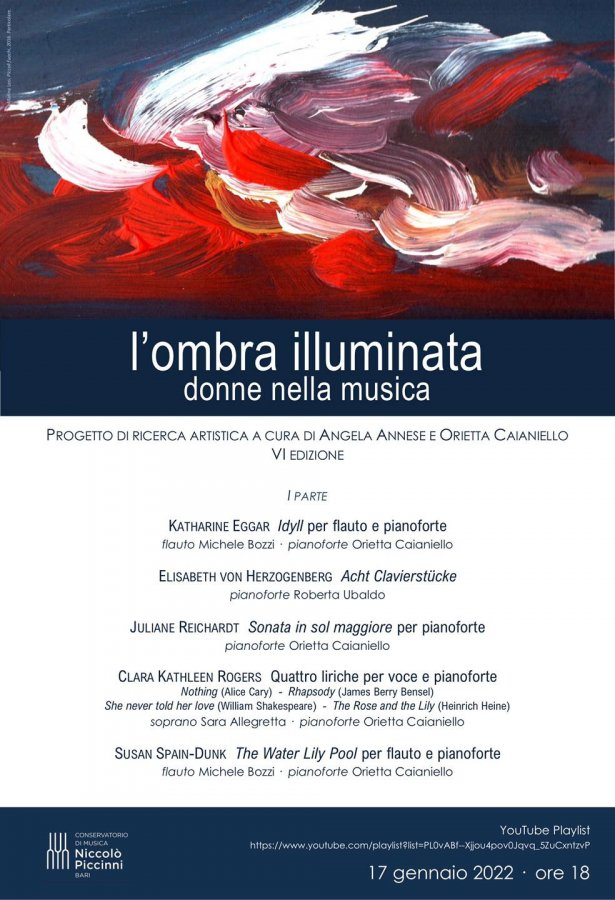
\includegraphics[width = .50\textwidth]{img/image1.jpeg}
			\caption {Locandina dell'evento}
		\end{center}
	\end{figure}
	
	\subsection{Sessione di registrazione}
	Effettuare una buona registrazione è fondamentale al fine di ottenere un buon prodotto finale, perchè una ripresa di qualità apre a semplici e funzionali possibilità di indagine e di lavoro del materiale, in termini di EQ, dinamica e stereofonia.
	
	\paragraph{Criteri di scelta}
	Una fondamentale premessa da fare è che non esistono specifiche regole, le scelte da prendere in fase di ripresa devono essere funzionali all'obiettivo che si vuole raggiungere, dunque è importante decidere il tipo di prodotto finale che si vuole ottenere, e di conseguenza pensare al come ottenere materiale ottimale da utilizzare a tal fine. In base a questo si prendono decisioni relative a:
	
	\begin{compactitem}
		\item \textbf{Scelta dei microfoni:} In base alla sorgente da riprendere e al ruolo che questa avrà nel mix finale, si scelgono i microfoni più adatti alla situazione tenendo conto di diversi parametri:
			\begin{compactitem}
				\item diagramma polare, ovvero la sua direzionalità: se si predilige ottenere un suono ambientale è meglio utilizzare un omnidirezionale, così da riprendere tutte le riflessioni dell'ambiente in uno specifico punto. Mentre nel caso in cui si intende riprendere il suono diretto, allora è preferibile utilizzare un cardioide, essendo un microfono con una direzionalità ristretta
				\item tipologia, scelta in base all'escursione dinamica della sorgente: se quest'ultima ha un'ampia escursione e la si intende mantenere, è preferibile utilizzare un microfono sensibile in modo tale che vengano ripresi anche i suoni a bassa intensità, come uno a consensatore.
			\end{compactitem}
		\item \textbf{Distanza dei microfoni dalla sorgente:} In base alle qualità del punto di registrazione principale, in un ensemble si identificano gli elementi qualitativi di una sezione precisa che mancano alla sua ripresa principale, al fine di bilanciare lo spettro e l'ambiente fornendo le informazioni mancanti avvicinando il microfono, come il dettaglio dello strumento o le alte frequenze.
	\end{compactitem}
	
	\paragraph{Mappatura dei microfoni}
	Il primo passo necessario per organizzare al meglio una sessione di post produzione audio di un concerto è indubbiamente lo studio dell'organizzazione dello spazio sul palco e della disposizione dei microfoni, al fine di comprendere gli aspetti qualitativi di ciascuna registrazione e poterli, di conseguenza, sfruttare al meglio ricostruendo una determinata immagine stereofonica in fase di post produzione audio.
	Nella sessione di registrazione, sono stati installati 3 punti di ripresa:
		\begin{compactitem}
			\item \textbf{Pianoforte} per questo punto di ripresa è stata utilizzata una coppia stereofonica Schoeps in configurazione ORTF, posta 30cm circa al di sopra della cordiera del pianoforte
			\item \textbf{Arpa} per questo punto è stato utilizzato un microfono omnidirezionale di marca Line Audio, modello OM1, posto a 30cm circa dalle corde dello strumento.
			\item \textbf{viola/soprano} per questi due elementi è stato utilizzato lo stesso punto di ripresa, ovvero un microfono cardioide di marca Line Audio, modello CM4.
		\end{compactitem}
	
	%inserisci uno screen del video dove si vede bene il palco e i microfoni

\section{L'approccio}
Una volta chiara l'organizzazione dello spazio acustico e l'interazione delle fonte sonore con i punti di ripresa, è bene avanzare determinate premesse generali per considerare problematiche comuni nel mondo della rappresentazione di una fonte sonora, ovvero: quanto la resa qualitativa finale potrà essere fedele alla realtà?

	\subsection{Problematiche assolute}
	Qualsiasi rappresentazione di un evento sonoro resta solo una rappresentazione. Ad oggi non esistono strumenti in grado di farci vivere un'esperienza immersiva come un concerto in una situazione non dal vivo. Siamo sottoposti a dei vincoli:
	
	\paragraph{Registrazione} Le fonti sonore acustiche non sono \textbf{puntiformi}, ma sferiche. Questo vuol dire che non è possibile rappresentarle con uno strumento di ripresa puntiforme come un microfono perchè, in quanto tale, può riprendere il suono da un solo specifico punto, senza costruire una totalità sonora come potrebbe un ascolto binaurale. Bisogna anche tenere conto della direzionalità del microfono, considerando che riprende il suono in maniera differente a seconda della sua provenienza, e non esiste, ad esempio, un microfono omni-direzionale che lo sia realmente a tutte le frequenze e quindi, lineare in direzionalità. C'è da precisare che anche le nostre orecchie sono dei transduttori non lineari: sia in termini di direzionalità, che da un punto di vista spettrale: la sensibilità del nostro apparato uditivo cambia a seconda delle frequenze che ci interagiscono; i microfoni, seppur non in egual modo, possiedono lo stesso "difetto".
	Tuttavia, spesso l'utilizzo che si può fare di uno strumento può fare la differenza: adoperare specifiche tecniche di microfonazione ponendo in interazione tra di loro diversi microfoni può portare a risultati strabilianti. Partendo da semplici tecniche stereofoniche come  le configurazioni AB o XY, sino ad arrivare a configurazioni complesse come un microfono Soundfield: un microfono composto da quattro capsule microfoniche cardioidi o sub-cardioidi disposte a tetraedro che permette di rappresentare un punto di ascolto in maniera sferica, ma in tal caso bisognerebbe comunque superare l'ostacolo della
	
	\paragraph{Riproduzione} Ovvero, potrebbe anche essere possibile riprodurre una registrazione catturata da un microfono Soundfield con un altoparlante tetraedrico, anche lui composto da più diffusori \textbf{puntiformi}, ma in tal caso comunque suonerebbe \textbf{un punto di ascolto} (con i suoi limiti dati dalla non-linearità dei microfoni e degli altoparlanti) e non \textbf{la fonte sonora originale}
	
%parla del vincolo di dover catturare una fonte sonora sferica o comunque non lineare con un  microfono. e di conseguenza del vicolo di dover riprodurre queste registrazioni con un impianto stereo, dunque da degli altoparlanti che rappresentano dei punti di diffusione non sferici, non reali, o comunque estremamente direzionali
	
	\subsection{L'obiettivo}
	Dato che l'evento ha avuto luogo in un auditorium estremamente curato nella sua acustica, l'obiettivo che mi sono posto è avvicinarsi quanto più possibile alla resa acustica originale. Tenendo conto comunque di non poter venir meno ai vincoli sovracitati, trattandosi di problematiche assolute.
	
\section{Gli interventi}
Nella fase di analisi del materiale all'inizio di una sessione di post produzione audio, emergono le problematiche principali che si dovranno affrontare al fine del raggiungimento dell'obiettivo principale. Questo è il momento fondamentale nel quale vanno prese delle scelte su diverse questioni.

	\subsection{Routing dei canali}
	Al fine di restituire un prodotto che abbia una resa fedele all'acustica dell'auditorium in questione, è importante effettuare un buon routing dei canali impostando delle buone basi di lavoro per poter gestire comodamente l'ambiente stereofonico: per questo motivo ho deciso di impostare, \textbf{laddove fosse possibile}, l'organizzazione dei canali in configurazione Mid/Side.
	
		\paragraph{ORTF} La registrazione dell'ORTF, essendo a due canali, permette di fare un routing Mid Side sommando L+R (e dimezzandone le ampiezze) nel primo canale della nuova traccia per ottenere il Mid, e L+(-R) (dimezzando anche quì le ampiezze) nel secondo canale ottenendo il Side.
		In questo modo, su specifiche DAW che ci permettono di lavorare separatamente su ciascun canale di una traccia, come ad esempio Reaper, posso lavorare separatamente sul Mid e sul Side. Questo apre la strada a numerose possibilità di indagine e di missaggio dell'immagine stereofonica in termini di ampiezza e dimensioni.
		
		\paragraph{Spot dell'arpa} L'arpa è uno strumento duttile, di carattere avvolgente e delicato. Per questo motivo mi sarebbe piaciuto avere un controllo specifico sulla sua dimensione, l'ideale sarebbe stato farlo tramite un routing  Mid/Side. Ma la registrazione dello spot monofonico dell'arpa non apre a questa possibilità perchè la sorgente è registrata in mono: questo non permette di effettuare un routing Mid Side perchè i canali L e R contengono fondamentalmente lo stesso identico segnale. Di conseguenza, sommare L+(-R) equivale ad ottenere cancellazioni di fase che cancellano totalmente il segnale non permettendo di ottenere la componente Side della sorgente. Sull'altro canale invece, altro non avrò se non una somma di due registrazioni identiche, ovvero L+R. Data la situazione, occorre limitarsi a lavorare solo sul Mid.
		
		\paragraph{Spot per viola e voce} In questo caso, come per l'arpa, abbiamo a che fare con un'unico spot monofonico addirittura per due sorgenti diverse, registrate in momenti diversi.
		Data la situazione e i limiti che ci impediscono di eseguire un'indagine stereofonica sul materiale, anche in questo caso occorre arrangiarsi e lavorare solo sul mid.
		Oltre questo, l'unica operazione valida da considerare è in termini di equalizzazione: si potrebbe copiare il materiale in due tracce diverse del mixer, in modo tale da poter equalizzare separatamente le registrazioni di viola e voce, dato che sopraggiungono in momenti differenti della performance
	
	\subsection{EQ}
	
	\subsection{Processori di dinamica}
	La dinamica è lavorabile, gli interventi da effettuare eventualmente dipendono dal carattere che si intende dare al prodotto finale. Sicuramente le sorgenti sonore registrate hanno una notevole escursione dinamica, ed occorre comprendere quali sono i punti e gli strumenti nei quali la si vuole mantenere, ma procediamo per gradi.
	
		\paragraph{Introduzione} è stata registrata, purtroppo, solo dallo spot omni dell'arpa, oltre che dal microfono integrato nella videocamera con la quale è stato ripreso l'evento. Questo vuol dire che il materiale a disposizione del parlato è solo ambientale e a basso volume, di conseguenza ho svolto due operazioni: anzitutto ho normalizzato a mano le clip effettuando dei tagli e impostando dei guadagni. Successivamente, è stata applicata una lieve compressione per portare tutto allo stesso livello e contenere le escursioni dinamiche tra parlato a suono degli applausi.
		
		\paragraph{Pianoforte} Avendo effettuato un routing M/S dalla registrazione del pianoforte, è possibile indagare e lavorare il materiale intervenendo separatamente su Mid e Side. In questo caso, applicare una leggera compressione al mid del pianoforte potrebbe aiutare a dargli una spinta in più, trattandosi dello strumento protagonista di tutta l'esecuzione. Ma come è possibile intervenite in maniera trasparente, in modo tale da non comprimere eccessivamente la dinamica? Una volta impostato un livello indicativo di Ratio (rapporto di compressione) utile a percepire il lavoro del processore, il primo parametro comodo sul quale lavorare quando si effettua una compressione è la treeshold, ovvero la soglia al di la della quale il compressore inizierà a lavorare. In questo caso la si può impostare 2/3 dB al di sotto del livello dei picchi massimi, in modo tale da comprimere poco materiale. Ma quanto viene compresso? Quì entra in gioco la Ratio, la quale funziona per frazioni: un rapporto di 2:1 tirerà fuori 2dB per ogni dB in input, e in questo caso potrebbe andare bene.
		Ora è il momento di scegliere il carattere della compressione tramite i tempi di atacco e rilascio. In questo caso l'obiettivo è di ottenere un risultato morbido e meno tagliente possibile. per rendere l'intervento trasparente si può impostare un tempo di attacco rapido (0.5ms) e un tempo di rilascio prolngato (>300ms).
		Tenendo conto che non intendo comprimere la dinamica alzando il materiale a basso volume, manterrò un gain a 0dB
	
\section{Conclusioni}

\begin{compactitem}
	\item Il miglior approccio per poter rappresentare al meglio una fonte sonora, è meditare sulla questione che, con i mezzi a nostra disposizione nella nostra epoca, siamo inevitabilmente posti dinanzi a dei muri invalicabili che ci separano da una rappresentazione di una fonte sonora che sia oggettivamente fedele alla realtà.
	E possibile però sfruttare al meglio determinati strumenti per restituire comunque un prodotto vivibile.
	\item Si inizia a lavorare al mix definitivo già dalla fase di registrazione: se le registrazioni sono state effettuate a dovere, l'ingegnere avrà un'ottima base di lavoro per post-produrre il progetto, dovendo intervenire in piccolissime dosi ed in maniera ottimale oltre che con estrema semplicità.
\end{compactitem}
	
	
%	\begin{figure}[h]
%		\centering
%		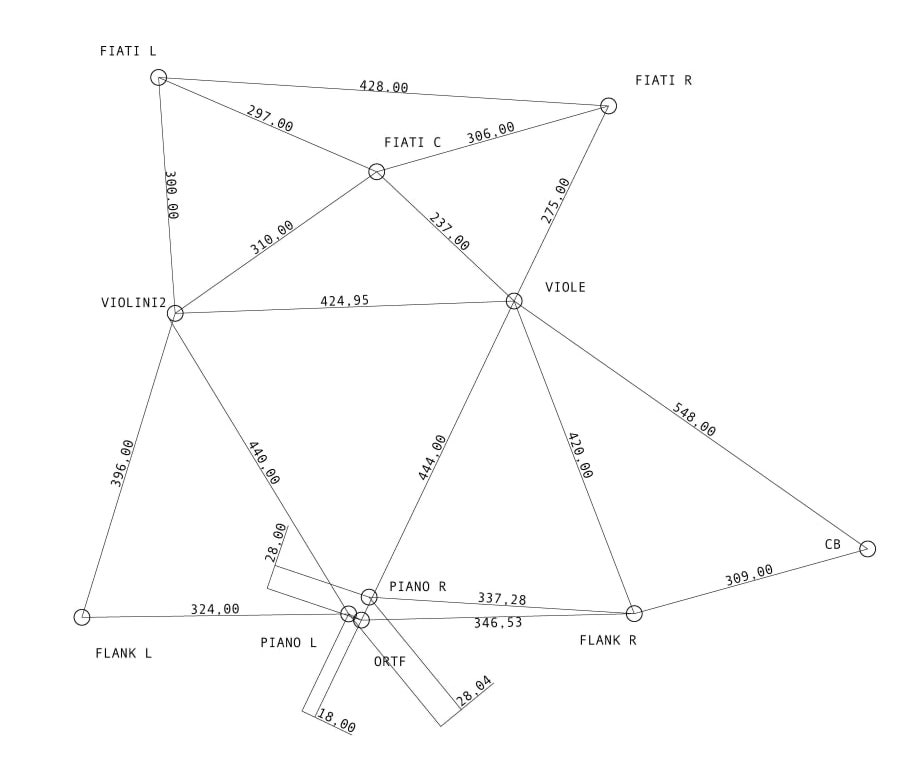
\includegraphics[width=.50\textwidth]{img/image2.jpg}
%		\caption{Mappa della disposizione dei microfoni realizzata da Gabriele Acquafredda}
%		\label{gs}
%	\end{figure}
	
	
	\vfill\null
	
	\newpage % USE NEWPAGE TO FORCE COLUMNN INTERRUPTION
	%-------------------------------------------------------------------------------
	%-------------------------------------------------------------------------------
	
	%--------------------------------------------
	%----------------larghezza massima del codice
	
	\vfill\null
	
	\raggedright
	%\bibliographystyle{unsrt}
	%\printbibliography
	
\end{document}

%%%%%%%%%%%%%%%%%%%%%%%%%%%%%%%%%%%%%%%%%%%%%%%%%%%%%%%%%%%%%%%%%%%%%%%%%%%%%%%%
% 2020 GIUSEPPE SILVI ARTICLE TEMPLATE BASED ON
%%%%%%%%%%%%%%%%%%%%%%%%%%%%%%%%%%%%%%%%%%%%%%%%%%%%%%%%%%%%%%%%%%%%%%%%%%%%%%%%
% Journal Article
% LaTeX Template
% Version 1.4 (15/5/16)
% This template has been downloaded from:
% http://www.LaTeXTemplates.com
% Original author:
% Frits Wenneker (http://www.howtotex.com) with extensive modifications by
% Vel (vel@LaTeXTemplates.com)
% License:
% CC BY-NC-SA 3.0 (http://creativecommons.org/licenses/by-nc-sa/3.0/)
%%%%%%%%%%%%%%%%%%%%%%%%%%%%%%%%%%%%%%%%%%%%%%%%%%%%%%%%%%%%%%%%%%%%%%%%%%%%%%%%
